% Todo:

\documentclass[12pt]{article}
\usepackage{hyperref}
\usepackage{xeCJK}
\usepackage{fontspec}
%\setCJKmainfont{SimSun}
\setCJKmainfont[BoldFont=SimHei,ItalicFont=KaiTi]{SimSun}
% \setCJKsansfont{SimHei}
% \setCJKmonofont{SimKai}
\setmainfont{Arial}

\usepackage{cite}
\usepackage{graphicx}
\usepackage{float}
\usepackage{amsfonts}
% \usepackage{amsmath}	% for \tag
\usepackage{amssymb}	% for \multimap
% \usepackage{stmaryrd}
\usepackage{color}
%\usepackage[square,numbers]{natbib}
%\nocopyright
%\usepackage{latexsym,amsmath,amssymb,graphicx,hyperref}
%\usepackage{times} % gives you a bit more space if needed
\usepackage{titlesec}		% change color of section headings
\usepackage{verbatim}

\makeatletter
\newsavebox{\@brx}
\newcommand{\llangle}[1][]{\savebox{\@brx}{\(\m@th{#1\langle}\)}%
  \mathopen{\copy\@brx\kern-0.5\wd\@brx\usebox{\@brx}}}
\newcommand{\rrangle}[1][]{\savebox{\@brx}{\(\m@th{#1\rangle}\)}%
  \mathclose{\copy\@brx\kern-0.5\wd\@brx\usebox{\@brx}}}
\makeatother

\titleformat{\section}
{\color{blue}\normalfont\Large\bfseries}
{\color{blue}\thesection}{1em}{}
\titleformat{\subsection}
{\color{blue}\normalfont\large\bfseries}
{\color{blue}\thesubsection}{1em}{}

\renewcommand\abstractname{\textcolor{blue}{Abstract}}

\definecolor{LogicColor}{rgb}{0.4,0.1,0.4}  % Magenta
% \definecolor{LogicColor}{rgb}{0,0,0}	% for black-and-white paper

\newcommand{\concept}[1]{\textbf{\textcolor{blue}{#1}}}

\newcommand{\english}[1]{\rmfamily \textit{``#1''}\rmfamily}
\newcommand{\formula}[1]{\textcolor{LogicColor}{#1}}

\newcommand{\df}{f} %probability density function
\newcommand{\dfo}{f1} %other probability density function
\newcommand{\fv}{x} %fuzzy variable
\newcommand{\tab}{\hspace*{1cm}}
\newcommand{\zand}{\; \tilde{\wedge} \;}
\newcommand{\zor}{\; \tilde{\vee} \;}
\newcommand{\PimpL}{\leftarrowtriangle}
\newcommand{\com}{\multimap}
\newcommand{\comL}{\circ \hspace{-0.4em} - \,}
\newcommand{\mul}{}
\newcommand{\loves}{loves }
\newcommand{\heart}{\, \heartsuit \,}

\newcommand*\sigmoid{\vcenter{\hbox{\includegraphics{sigmoid.png}}}}
\newcommand*\sadface{\includegraphics[scale=0.25]{face-sad.png}}

\setlength{\oddsidemargin}{1cm}
\setlength{\evensidemargin}{1cm}
\setlength{\textwidth}{14cm}

\title{\textcolor{blue}{Genifer 4.1 theoretical notes}}
\author{YKY (\textit{甄景贤})}
\date{27 May 2015}
% \institute{}

\begin{document}

\tab\tab\tab \parbox{9cm}{\textit{The ultimate goal of mathematics is to eliminate any need for intelligent thought.}}
% \vspace{-0.5cm}
\begin{flushright}
\textemdash\, Alfred North Whitehead \hspace{1cm}
\end{flushright}

\sffamily

{\let\newpage\relax\maketitle}

\maketitle
\setlength{\parindent}{0em}
\setlength{\parskip}{1.5ex plus0.5ex minus1.2ex}

\begin{comment}
\noindent 本文介绍人工智能 Genifer4 的理论,特别是对数学专业的人。 Genifer4 的目的是将 logic-based AI (例如 OpenCog, NARS, Genifer3) 转移到向量空间的架构下,令我们可以使用「连续」的技巧,例如算子、迭代法、梯度下降等。 这些技巧可能比较快。
\end{comment}

For readers curious about what I'm doing in Genifer 4, it is really not a big deal, basically I am trying to transfer logic to a \textbf{continuous setting}, so that I can apply iterative approximation techniques, such as gradient descent.

In the past year, after a Herculean effort, I barely succeeded in making logic continuous (and even this part is fraught with problems), but at least the problem of inductive learning seem to be transformed into one of mathematical continuous optimization.

And then I discover, the most efficient optimization methods are based on convex technologies.  As in the following figure, the fitness landscape above is convex, the one below is non-convex: \footnote{from Charles H Martin's \href{https://charlesmartin14.wordpress.com/2013/11/14/metric-learning-some-quantum-statistical-mechanics/}{blog}.}
\begin{figure}[H]
\centering
\includegraphics[scale=0.6]{convex-and-nonconvex.jpg}
% \caption{Convex and non-convex fitness landscapes.}
\end{figure}

If we don't assume convexity, we have to fall back on techniques like genetic algorithms, branch-and-bound, etc.  Those techniques I have already known for a long time in computer science, so I disappointedly felt my efforts have been in vain \sadface

The latter algorithms could still be fast, but they are \textit{heuristics} which means there are no speed gaurantees.  Because the complexity of inductive learning is extremely high, do we dare to try the heuristics?  For instance, would you risk investing \$10,000's to bet on Genifer 3.0?

Mathematics is truly wonderful, it progresses constantly, but sadly it progresses very slowly.  Right now I see the frontier is to extend convex optimization, but I have not seen any great breakthroughs (though I am just a novice and have not surveyed the entire field.)  If there is indeed such a breakthrough, it would really be ground-breaking, but that is not something within  the capacity of ordinary folks, not even a lot of professional mathematicians.

Right now what we could do is probably:
\begin{itemize}
\item find a problem that is non-convex but which could still be solved efficiently, then transform our problem to that problem.
\item change the representation of the original problem;  this requires innovative thinking.  Or even turn the optimization problem into an equation solving problem, etc.
\item then see if the fitness landscape might have some better characteristics;  This requires experimentation, plotting those error surfaces.
\item give up convexity, we could still use other global optimization techniques:  genetic algorithms, branch-and-bound, convex-concave / DC programming, back-propagation for neural networks, simulated annealing, etc.  As I said, some of these techniques do not need continuity, we can go back to Genifer 3.
\end{itemize}

In the remaining article, I will talk about my attempt at making logic continuous, which might still find a use some day (but then again could also be a dead end).

\section{Making logic continuous}

Basically I try to establish this correspondence:
\begin{center}
\colorbox{yellow}{\parbox{0.95\textwidth}{
\begin{tabular}{ccc}
KB (knowledge base) & $\Leftrightarrow$ & vector space \\
logic rules & $\Leftrightarrow$ & non-linear operators \\
learning logic rules & $\Leftrightarrow$ & searching for operators in functional space \\ 
\end{tabular}
}}
\end{center}

Even after the transition to continuous there would still be the non-convexity problem, we don't bother now.  Just making it continuous is hard enough, because the structure of classical logic is very complicated.

Many theories of logic are expressed in mathematical symbols, but they actually do not have strong connections with other existing branches of mathematics, so they are no more than a pile of symbols.  To be truly useful, we have to build \textit{bridges} to other branches of mathematics.  I find that it is easiest to do via (abstract) algebra, as the algebraic formulation allows to easily see similar patterns in other areas.

\section{What is logic?}

Logic can be divided into \concept{propositional logic} and \concept{predicate logic}, the former is isomorphic to Boolean algebra and is easier to understand and mathematically simpler;  The latter is difficult to model mathematically, for example it requires using the \textit{cylindric algebra} invented by Tarski, that is little known outside of the logic circle.  I am trying an alternative route based on \textbf{combinatory logic} and \textbf{relation algebra}. \footnote{Combinatory logic changes the predicate logic form $R(a, b)$ to the algebraic form $R \,a\, b$ or $a \,R\, b$, for example $loves(john, mary)$ is changed to $john \cdot loves \cdot mary$.  Relation algebra is a special form of combinatory logic.}

% 很多数学专业的人没有时间钻研 predicate logic,所以我很寂寞,但我希望你们能暂时忽略一些 details,而我们可以尽量讨论一些具体的数学问题。

Firstly, it is obvious that logic formulas can be expressed as tree structures, and trees in turn can be easily expressed in sum-product algebraic form.  For example (this is even a binary tree):
\begin{figure}[H]
\centering
\includegraphics[scale=0.5]{logic-formula-tree.jpg}
% \caption{Convex and non-convex fitness landscapes.}
\end{figure}

However there is difficulty in expressing this in vector space.  Vectors can be added but there is no obviously good candidate for vector multiplication.  For example, if two unrelated formulas such as \formula{john$\cdot$loves$\cdot$mary} and \formula{paul$\cdot$loves$\cdot$playing$\cdot$basketball} end up ``crashing'' into each other in \concept{conceptual space}, or being in proximity without any real reason, would be troublesome for the system.

\section{Cayley graph}

Earlier I tried an idea using the Cayley graph, but I found that it has many difficulties.

The idea of Cayley graph is very simple, for example the following diagram is the free group generated by 2 elements $\{ a, b \}$, the products are linked by edges:
\begin{figure}[H]
\centering
\includegraphics[scale=0.25]{cayley-graph.jpg}
\end{figure}

There is also the notion of \concept{ontology} in AI, for example: \formula{cats $\subseteq$ animals}.  Ontology can be expressed as a hierarchical cluster, which can be shaped as a circle or ball:
\begin{figure}[H]
\centering
\includegraphics[scale=0.5]{ontology-ball.png}
\end{figure}

I attempted to combine the ideas of Cayley graph and ontology:  In the Cayley graph each node is a \concept{concept} (eg \formula{love} or \formula{football}), and every concept can find its location in the ontology ball.  But the ontology ball itself is hierachically structured, and it seems difficult if I try to "embed" it into Cayley graph nodes.

Moreover, as the Cayley graph's number of branching increases, it looks more and more "unnatural";  for example this is the case for just $n=5$:
\begin{figure}[H]
\centering
\includegraphics[scale=0.25]{cayley-graph-5.png}
\end{figure}
The reason is that Cayley graphs are actually fractal structures!  I have wished to achieve the "continuous" effect, but in the Cayley graph jumping from node to node is \textbf{discontinous}.

Nevertheless, Cayley graph has another advantage, that it can be embedded into the hyperbolic disc, which possesses the metric of \textbf{hyperbolic geometry}  (as seen in many of M C Escher's artworks, ie, the metric shrinks as we move closer to the edge of the disc):
\begin{figure}[H]
\centering
\includegraphics[scale=0.75]{hyperbolic-disc-beautiful.png}
\end{figure}

In hyperbolic geometry straight lines turns into arcs, and in artificial neural networks the discriminant function also contains the linear form $Y = \sigmoid(\sum W_i X_i)$, so perhaps we can create a kind of "hyperbolic neuron"?  Unfortunately due to the discontinuity issue, this idea is abandoned for now.

\section{Distributive vector representation (DVR)}

This is a better approach, and seems to solve the \textbf{continuity} issue.

Under DVR, knowledge is represented by a very long vector:
$$ K = \mathbf{v} = (v_1, v_2, ... , v_n) $$
as is quite common in neural networks.  This means that each \textbf{concept} is not represented by a single neuron (= a single $v_i$), but rather by an entire layer of neurons (= $\mathbf{v}$).   Under this representation, a concept is one or more \textbf{regions} in space, and the regions can be disjoint.

For example, when the dimension of the vector space is $n=2$, we can have an example like this:
\begin{figure}[H]
\centering
\includegraphics[scale=0.5]{distributive-vector-representation-en.png}
\end{figure}

Vectors can be \textbf{added}, where addition means \concept{superposition}, which notion came also from neural networks.  For example, the two formulas: \formula{john$\cdot$loves$\cdot$mary} and \formula{pete$\cdot$loves$\cdot$football} can be superimposed on $K$, meaning that both sentences are simultaneously true.  As long as concepts do not "crash" into each other, this is feasible.

But there is still another problem:  when a formula is repeated, its truth value would not be doubled (as when I repeat "john loves mary" twice);  In other words, $a \wedge a = a$, but in vector addition this will be doubled, unless we use vector space over a special \textbf{field} where $ 1 + 1 = 1 $ or something\footnote{ One may use the "tropical" semi-ring, or min-plus algebra.}.  This is a detail to be treated later.

For now we skip the issue of \textbf{multiplication}.  In \S 7 we discuss how to handle products.

\section{Deduction in logic}

The most basic operation in logic is to \textbf{deduce} a new formula from the KB (\concept{knowledge base}).  The ``KB'' terminology came from classical AI, we denote it simply as $K$ in the new formulation.

The basic operation of deduction is to \textit{apply rules to facts}.  Deduction can be represented by the operator $T$:
$$ T: K \mapsto K .$$
But $T$ is \textbf{non-linear}.

$T$ corresponds to one logical rule.  A classic example is the definition of ``granddaddy'':\\
\tab \formula{ granddaddy(X,Z) $\leftarrow$ daddy(X,Y) $\wedge$ daddy(Y,Z)}

To perform this deduction step, we need to perform \textbf{pattern matching} first, and then the rule can be \textbf{applied} to matched facts.

So we have this correspondence:
\begin{center}
\colorbox{yellow}{\parbox{0.55\textwidth}{
\begin{tabular}{ccc}
deduction & $\Leftrightarrow$ & apply operators \\
pattern matching & $\Leftrightarrow$ & filter: $K \rightarrow K$ \\ 
\end{tabular}
}}
\end{center}

For example, assume we know the following facts:\\
\tab \formula{daddy(john, pete)} \\
\tab \formula{daddy(pete, paul)} \\
and we need to find the substitution \{ john/X, pete/Y, paul/Z \}, in order to apply the above rule.  Finding this substitution is called pattern matching; the classic \textbf{unification algorithm} accomplishes that.

That is the reason why $T$ is \textbf{non-linear}:  For various $K$'s, the action of $T$ is usually 0, unless pattern matching succeeds, then $T$'s action would be non-zero.  (Of course, we would make $T$ smooth, so the "= 0" above would be replaced with "close to 0".)

In an AI system there would be many rules $T_1, T_2, ...., T_n$.  Applying $T_i$ on the KB, superimposing them together, that would be a \textbf{single step} of deduction.  But because $T_i$ is non-linear, the summation and $T_i$ do not \textbf{commute}.

A single step of deduction is:
     $$ K' = \sum T_i (K) $$
and the \textbf{full logical consequence} of the KB is:
\begin{eqnarray} \nonumber
K^\infty & = & \mbox{the above step repeated infinitely} \\ \nonumber
         & = &  (\sum T_i) ^\infty (K) .
\end{eqnarray}

\section{Learning}

The learning algorithm is the bottleneck of AI.  If we have a good inductive learner, other details are just details (say we can solve with \textbf{reinforcement learning}).

The special thing about logic-based learning is that it has a \textbf{doubly iterative} structure that consists of \textbf{deduction} and \textbf{induction}.  Induction needs to call deduction, but deduction is itself a process of high complexity.

In other words, we first use deduction to get $K^\infty$ (this requires iteration of the operators):
$$ K^\infty = (\sum T_i) ^\infty (K^0) .$$
And then we compare the result $K^\infty$ with the ideal $K^*$, get the error, and our objective is to find a set of $T_i$'s to minimize the error.  The $T_i$'s live in a space of non-linear operators.

Logically what we aim at is:
$$ K^0 \cup \{ T_i \} \models E $$
where $E$ is the new examples or "new experience" that needs to be explained.  The idea answer is $K^* = K^0 \cup E$.

The error $\mathcal{E}$ is the difference between the deduced $K^\infty$ and the ideal $K^*$:
$$ \mathcal{E} = K^\infty - K^* = (\sum T_i) ^\infty K^0 - (K^0 + E) . $$

If the $T_i$'s are differentiable, the gradient $\partial\mathcal{E}/\partial T_i$ exists, and we can use gradient descent.

Compare this with ordinary optimization techniques, such as the Newton-Raphson, which is just the iteration of an operator:
$$ x^\infty = T^\infty x^0 $$
and $x^\infty$ would be the required answer.

Compare with the traditional back-propagation for neural networks.  The back-prop algorithm is:\\
\tab (a single neuron) \tab\tab $y_j = \sigmoid( \sum W_{ij} x_i )$ \\
\tab (multi-layer structure) \tab $\mbox{output} = y_0 \circ y_1 \circ ... \circ y_n (\mbox{input})$ \\
\tab (update rule) \tab\tab\tab $ \mathbf{W}' = \mathbf{W} + \alpha \; \partial \mathcal{E} / \partial \mathbf{W} $

In comparison:
\begin{itemize}
\item In back-prop the operators $ y_0 \circ y_1 \circ ... \circ y_n $ come from the many layers of neurons, so back-prop can be regarded as the propagation of errors in \textbf{space}.
\item Our iteration occurs in \textbf{time}, but that seems to make no essential difference.
\end{itemize}

My current diagnosis of the problem is:  The space of $K$ may be too large (though its dimension may not be so), because it contains all logic formulas, and if there is no approximation, this problem is exactly the same as the original logic learning problem, and there would not be any improvement, it would at best be a relaxation of the original.  We should exploit function approximation to achieve some \textbf{generalization}.

But logic has its own generalization structure.  The purpose of generalization is \textbf{compression}; we could as well say that learning is \textbf{compression}.  Logic-based learning itself is a compression scheme of very high complexity (which is why it's so slow).  The $A \subseteq B$ subsumption relation establishes a hierarchical classification structure, this classification amounts to \textit{taking the logarithm of the size of the knoweldge base}, just like we do in \textbf{binary search}.  However, due to the doubly exponential complexity of logic learning, perhaps this trick alone is not enough?

Stephen Muggleton, a leading researcher of inductive logic learning, wrote in a 2002 paper on applying \textbf{generic algorithms} to logic learning:
\begin{quote}
\textit{"The usual way for evaluating a hypothesis in first-order concept learning systems is to repeatedly call a theorem prover (eg Prolog interpreter) on training examples to find out positive and negative coverage of the hypothesis.  This step is known to be a complex and time-consuming task in first-order concept learning.  In the case of genetic-based systems this situation is even worse, because we need to evaluate a population of hypothesis in each generation.  This problem is another important difficulty when applying GAs in first-order concept learning."}
\end{quote}

\begin{comment}
压缩的方法必须是 ``semantic distance preserving'',意即: 在语义空间中相似的点被压缩到相邻的逻辑範式。

问题似乎是: 法则的诱导似乎不能单是基於语法。 概念阶层的诱导是基於: Liebniz 和 $a\, R\, b$。

Liebniz extensionality:
\begin{eqnarray}
xZ \rightarrow yZ \Leftrightarrow x \supset y \\
Zx \rightarrow Zy \Leftrightarrow x \supset y
\end{eqnarray}

The relation of subsumption is \textit{intrinsic} to the logic.  
\end{comment}

\section{Product structure}

I'm still unsure how to represent products, such as \formula{john$\cdot$loves$\cdot$mary}.

One proposal is from Geoffrey Hinton:  Each concept is a \concept{matrix};  If the concepts $a$ and $b$ are related by $a\, R\, b$, then their representing matrices would obey $ AR = B $, and the positions of such matrices in matrix space have to be learned.  This method seems a bit troublesome, as we need to perform the matrix multiplications to obtain which elements follow which.

A second proposal uses the \concept{tensor product}, but the tensor product space has high dimension that grows with the product's length.  Paul Smolensky's book \textit{The Harmonic Mind} (2006) volume 1 describes his distributive tensor product representation (which I will explain when I have time).

A third proposal is from the collection of papers \textit{Quantum Physics and Linguistics} (2013).  There they use \concept{monoidal categories}, a kind of categories that have products as well as compositions.  Its definition has:
\begin{itemize}
\item objects: $X, Y, ...$
\item morphisms: $f: X \rightarrow Y$
\item composition: $f \circ g : X \rightarrow Z$
\item grouping objects into: $X \otimes Y$
\item a special object for the ``empty system'': $I$
\item parallel composition: for $f_1: X_1 \rightarrow Y_1$ and $f_2: X_2 \rightarrow Y_2$ \\
\tab \tab $f_1 \otimes f_2: X_1 \otimes X_2 \rightarrow Y_1 \otimes Y_2$
\end{itemize}
Its algebraic operations can be represented by certain \concept{braid} diagrams:
\begin{figure}[H]
\centering
\includegraphics[scale=0.75]{frobenius_algebra.jpg}
\end{figure}
This seems to be a very general structure (including tensor products?)  A main theme of the book is that these categories are capable of covering all syntactic structures in natural langauge.  I don't have the time to study it in depth yet.

Another proposal is my invention.  The idea is:  we can treat the following function as a continous \textbf{time series}:
\begin{figure}[H]
\centering
\includegraphics[scale=0.75]{continuous-time-sequence-en.png}
\end{figure}
A product is a discrete sequence, we can make it continuous as a \textbf{curve} parametrized by $t$.

These curves in the space of $K \times t$ may look like this:
\begin{figure}[H]
\centering
\includegraphics[scale=0.75]{polynomial-hairs.png}
\end{figure}

The curves can be represented by splines, that are \concept{polynomials}.  Then perhaps we could apply tools in \textbf{algebraic geometry} (a highly sophisticated branch of modern mathematics).  A polynomial can be represented by its coefficients, ie, a list of numbers, which is very convenient.   And the map between polynomials are also polynomials, forming a \concept{dual space}, that reminds of the situation in logic, where formulas can apply to other formulas.

\section{Formal power series}

A power series has the form:
$$ \sum k_i a^i $$
but if the $a_i$'s are not ordinary numbers, the summation cannot be performed with ordinary addition, so we call it a \concept{formal series}.

Abstractly speaking, let $A$ be a set of \textbf{atomic concepts}, such as
$$\{ \, \mbox{love}, \mbox{hate}, \mbox{men}, \mbox{women}, ... \}$$
$A^*$ is the set of all sentences that can be combined from these concepts.  Multiply these sentences with some coefficients, for example:\\
\tab 0.8 \formula{john$\cdot$loves$\cdot$mary} + \\
\tab 0.3 \formula{mary$\cdot$loves$\cdot$john} + \\
\tab 0.9 \formula{mary$\cdot$loves$\cdot$pete} + \\
\tab ... \\
The coefficients $k_i \in K$ and $K$ can be an arbitrary \concept{semi-ring}.  We can regard $K$ as the semi-ring of \textbf{logical truth values}.

Denote all formal series like the above as $K\llangle A\rrangle$.

Formal series are closely related to \concept{finite state machines} (FSMs): FSMs can recognize \textbf{formal languages}.  A formal language $L$ can be any subset of $A^*$.  If $L$ contains a sentence, give it a coefficient 1, otherwise coefficient 0.  So we obtain a formal series representing that formal language.

Not all formal languages can be recognized by FSMs.

If recognizable, then for each letter (our ``atomic concept'') in this language, we can construct a $M_{n \times n}$ matrix, whose $M_{pq}$ entry depends on whether there is a state transition from $p$ to $q$ (1 if yes, 0 if no).

The multiplication of these matrices preserves the monoid multiplication rule, for example: $a \cdot b \cdot c \,\times\, d \cdot e \cdot f = a \cdot b \cdot c \cdot d \cdot e \cdot f$.

In \concept{representation theory}, we say this is a \textbf{matrix representation} of the monoid.

According to representation theory, multiplying a ring $K$ by a monoid $A$ gives us a $K$-module, so $K \llangle A \rrangle$ can be regarded as a (left) $K$-module.

Existence of the module implies existence of a representation.  (The famous Jewish woman mathematician Emmy Noether pioneered the use of modules to study representations.)

And we have just seen, FSM recognizable $\Rightarrow$ can build matrix representation.

So, "FSM-recognizable" is equivalent to "matrix representation exists", and this in turn is equivalent to "existence of a certain finitely generated $K$-submodule, that contains $S \in K \llangle A \rrangle$ (where $S$ is the formal series of the formal language).

Part of the above is from \textit{Encyclopedia of mathematics:  Noncommutative rational series with applications} (2011 Cambridge Univ Press).

\begin{center}
\colorbox{yellow}{\parbox{0.9\textwidth}{
\begin{tabular}{ccc}
% ??? logic formulas & $\Leftrightarrow$ & algebra over the ring of truth values \\
facts (propositions) & $\Leftrightarrow$ & monoid words \\
KB & $\Leftrightarrow$ & formal series \\
rules & $\Leftrightarrow$ & non-linear operators acting on formal series \\
\end{tabular}
}}
\end{center}

\section{Memory registers}

Lastly, I have to mention this:  The structure of classical logic is just too complex, our troubles are still not finished... 

In the Genifer 3 white paper, I explained that we need to introduce a logic with ``memory registers''.  In other words, we need to add some logical ``actions'', that allow to read and write those registers.

\begin{center}
\colorbox{yellow}{\parbox{0.85\textwidth}{
\begin{tabular}{ccc}
memory register & $\Leftrightarrow$ & vector space $K \times t$ \\ 
actions & $\Leftrightarrow$ & some meta-operations (?) over registers\\
\end{tabular}
}}
\end{center}

This is just too much trouble, perhaps I'll stop here and update next time, z\`{a}iji\`{a}n!

\begin{comment}
\section{徵求合作者}

例如,我去过 香港科技大學 找人,但那研究生说他们簽了合约,规定不准幫外面工作(大概这是大学控制知识产权的一种措施)。

\begin{tabular}{|c|c|c|c|}
\hline
\textbf{Notation} & \textbf{Meaning} & \textbf{Example } \\
\hline
$A \supset B$ & concept A is a superset of concept B &
$animals \supset cats$ \\
& &  \english{cats are animals} \\
\hline
$A \ni B$        & concept A contains an element concept B &
$a \circ bird \supset tweety$ \\
& & \english{Tweety is a bird} \\
\hline
$A \rightarrow B$ & proposition A entails proposition B &
$bird \, X \supset can \, fly \, X$ \\
& & \english{If X is a bird X can fly} \\
\hline
\end{tabular}

\begin{figure}
\centering
\includegraphics[scale=0.8]{ontology-relations-relations.pdf}
\caption{Left: relations between ontological data.  Right: a random example of dendrogram.}
\label{fig:ontology-relations-relations}
\end{figure}

\section*{Appendix: XXXX}

\section*{Acknowledgments}

I am heavily indebted to Pei Wang \cite{Wang2006} \cite{Wang2013} and Ben Goertzel \cite{Goertzel2011} for their seminal contributions to AGI.  To Abram Demski and Russell Wallace -- we have spent years exploring many ideas in logic.  Also thanks to Matt Mahoney, Jeff Thompson for discussions of the draft.  William Taysom, Seh, and Joseph Cheung helped implement the code.
\end{comment}

\bibliographystyle{plain} % or number or aaai ...
\bibliography{AGI-book}

\onecolumn

% Bigger figures

\end{document}
